%
% File hicss51.tex
%
% Contact: Holm Smidt, hsmidt@hawaii.edu
%%
%%
%% Based on the style files for ACL 2015 by 
%% car@ir.hit.edu.cn, gdzhou@suda.edu.cn


\documentclass[10pt]{article}
\usepackage[T1]{fontenc}
\usepackage[latin1]{inputenc}
\usepackage[table]{xcolor} 
\usepackage[letterpaper]{geometry}
\usepackage{hicss51}
\usepackage{times}
\usepackage[none]{hyphenat}
\usepackage{url}
\usepackage{latexsym}
\usepackage{minted}
\usepackage{graphicx}
\graphicspath{{images/}}

\newcommand{\sansserifformat}[1]{\fontfamily{cmss}{ #1}}%

%\setlength\titlebox{5cm}

% You can expand the titlebox if you need extra space
% to show all the authors. Please do not make the titlebox
% smaller than 5cm (the original size).


\title{An Explicative and Predictive Study of Employee Attrition}

\author{Nesreen El-rayes\\
  MTSM at NJIT \\
  {\underline{nde4@njit.edu}} \\\And
  Michael Smith\\
  MTSM at NJIT \\
  {\underline{mes6@njit.edu}}\\\And 
  Stephen Taylor\\
  MTSM at NJIT \\
  {\underline{smt@njit.edu} (Corr. Auth.)} \\}

\date{}

\begin{document}
\maketitle
\begin{abstract}
WRITE THIS IN THE END
\end{abstract}

\section{Introduction}
Building and maintaining a stable, productive, collaborative, and high-quality workforce is a primary concern 
for the majority of managing principals as success in this area tends to be a key factor contributing the 
overall firm prosperity [CITATIONS??].  Inevitably, all firms will experience employee attrition.  
Involuntary attrition is often the result of profitability and performance pressures, department or business 
line obsolescence, and mergers and acquisitions, among other factors [CITATIONS??].  In contrast,
voluntary attrition is driven predominately by employee concerns [CITATIONS].  Such considerations 
my focussed around, but not limited to, managerial direction, compensation and benefits, firm culture, 
firm desirability and location, promotion potential as well as non firm specific motivations, e.g. medical 
conditions or retirement. 
  
A central objective of the majority of human resource departments is to understand the root causes 
behind voluntary employee attrition and develop an associated mitigation strategy.  Effectively 
navigating such issues generally resulted in explicit positive monetary effects stemming from increased 
firm revenue and cost reductions manifested through the work retained highly performant employees. 
In addition, identifying and resolving issues found to be common to employee attrition often implicitly 
enhances firm culture and workplace desirably which in turn enables the recruitment of higher quality 
staff which further improve retention, firm operation, and business practices.  
We feel that the compounding effect nature of 
this employee attrition feedback loop on the overall success or failure of the firm is the essential motive 
for conducting a through investigation into this matter. [MORE CITATIONS FOR THIS PARAGRAPH]  

Traditionally, employee attrition and retention issues tend to examined through qualitative and anecdotal 
measures.  Specifically, human resources staff tend to conduct exit interviews after an employee provides 
a resignation notice in order to ascertain the motivations behind the decision to leave.  Although 
these conversations may be direct and candid, i.e. in the event an employee is leaving for a significantly 
more senior role or needs to change geographic location for family reasons, in actuality, human resources staff
encounter considerable difficulty discerning the employee's actual rationale.  By way of example, employees 
seldom offer negative criticism of management during exit interviews for fear of future personal retribution 
or inadvertent retaliation towards their close colleagues who will still remain at the firm.
These circumstances impact the employee attrition data aggregation and quality assurance process 
by making it cumbersome, at a minimum, which leads to additional difficulties determining which 
attrition issues should be of primary importance for management to resolve. In addition, employee 
attrition data is typically high confidential and only accessible to key stakeholders internally 
within a firm.  This fact has been a major impediment for the progression of academic research on 
this topic. [CITATIONS] 

Recently, internet based platforms such as GlassDoor and LinkedIn oriented towards working 
professionals have amassed large quantities of publicly available information related to individual 
employee resumes including employment history, frank reviews of firm culture, desirability, and management
as well as anonymous feedback.  Although this data often lacks attritional motivation information at 
the individual employee level, when combined with aggregate firm culture and management rankings, 
one may glean a number of insights into the collective behavior and motivations behind individual 
decisions to transition to a new employer. Our major aim is precisely in this vein.  More specifically, 
we conduct a quantitative data analysis of employee attrition motivations as well as develop 
predictive models that will enable human resources staff identify employees whose firm separation 
may be imminent.

We extend the work of \cite{Smart2016} who examine employee attrition and retention issues based upon 
a collection of approximately five thousand anonymously submitted resumes to Glassdoor.  We provide 
SUMMARY OF DATA ANLAYSIS EXTENSIONS.  In addition, SUMMARY OF NEW MODELS. Lastly, we delineate 
future data acquisition, analysis and model development extensions that we seek to investigate 
in future work. 

This article is organized as follows ... TYPE WHEN FINISHED 

\section{Data Description and Feature Engineering}

We first turn to describing the content extracted from a collection of 
employee resumes that will form the basis for the subsequent attrition studies. 
Next, we provide a variety of summary statistics of this information that 
are relevant for the design of latter predictive models.  Then we discuss 
our data normalization process and 
several features constructed from this original data which will be utilized 
as input into these models.
In addition, we outline limitations of this dataset and ideas for improvement  
in future work.

\subsection{Data Source Description}

We worked in conjunction with the authors of \cite{Smart2016} to obtain 
a collection of 5550 examples of employee job transitions between 
2007 and 2016 which were sourced from an extensive proprietary database of 
resumes shared anonymously though Glassdoor's platform.  A job transition 
is define to be any instance of an employee listing a new role on their 
resume which may be associated with the present or original or a new employer
designated as internal and external moves.  Internal moves are typically 
significant in the sense of the employee either changing roles or 
being promoted within an organization as opposed to being reassigned 
within a current team. External moves are of interest for our 
attrition studies as in this situation employees leave their original 
firm entirely.

We summarize several salient features of the dataset construction process 
and expound upon details relevant to model development below; we refer the
reader to \cite{Smart2016} for a complete description of the data source. 

Each employ job transition contains 45 attributes.  Relevant attributes 
include employee specific information. Namely, a binary identifier 
indicating if the employee remained within or left their original firm,
the start and end dates of employment at the original firm, the 
employee's average salary during their tenure with the original employer, 
and the employee's job title. 
In addition, each transition includes employer related information. 
Specifically, employer name and metro location, the industry sector of which the employer 
is a member, the founding year of the firm, and the total number of employees. 
Finally, employer rating information is included.  Particular ratings are 
given for the following GlassDoor created categories: overall, firm CEO, friend recommendation 
business outlook, career opportunities, compensation and benefits, culture and values, 
worklife balance, and senior management. 
We note that in the event the employee transitioned to a new firm, when applicable,
the above information specific to both the original and new employer is present in this dataset. 
Finally, this dataset if fully populated with the exception of missing values in 
approximate 6\% of the original and new employer founding year values, respectively;
such null values are disregarded 
only in studies that depend upon this variable below.

\subsection{Summary Statistics, Feature Engineering and Data Normalization}

\begin{enumerate}
    \item percentage increase in salary 
\end{enumerate}


A total of 1429 employees remained at their present firm whereas 4121 
transitioned to a new firm.

\begin{figure}[thb]
    \centering
	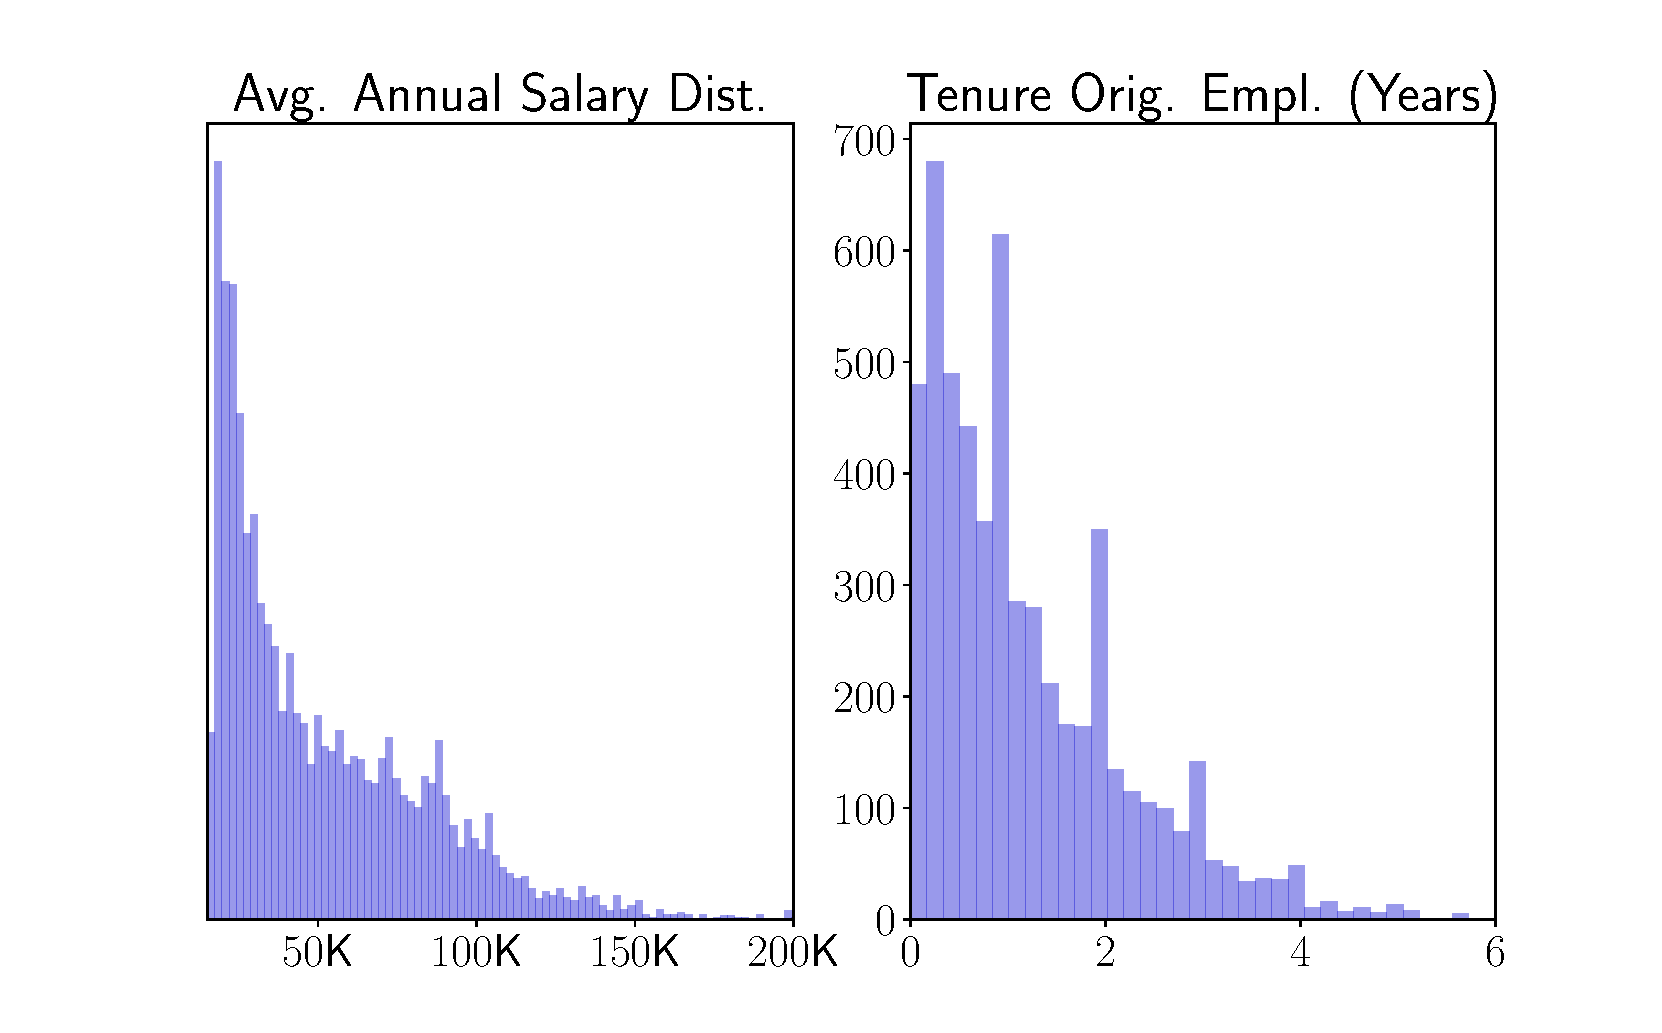
\includegraphics[width=1.0\linewidth]{avgsal.pdf}
    %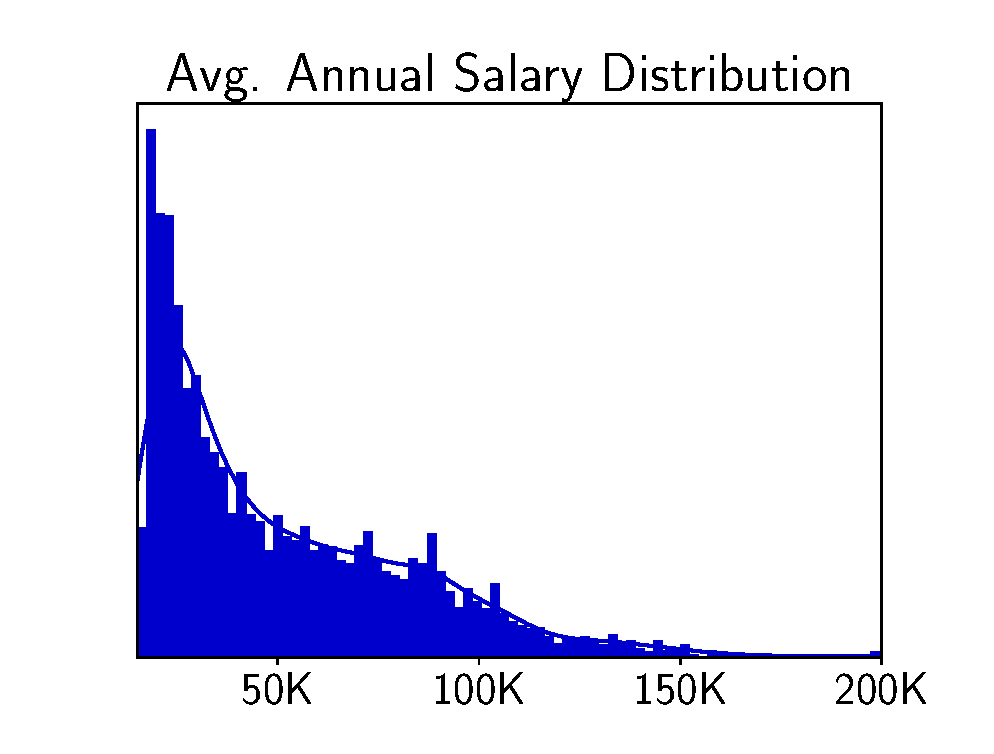
\includegraphics[trim={3cm 3cm 3cm 3cm}, clip,width=0.9\linewidth]{avgsal.eps}
	\caption{Employee average salary and tenure distribution at Original employer}
	\label{fig:avgsal}
\end{figure}

\begin{table}
  \rowcolors{2}{gray!25}{white}
  \centering
  \caption{Transition Counts Per Industry}
  \begin{tabular}{cccc}
    \rowcolor{gray!50}
      Industry & Cnt. & Industry & Cnt. \\
      Retail & 1357 & Manufact. & 191\\
      Education & 766 & Insurance & 144\\
      Info. Tech. & 718 & Media & 113\\
      Finance & 590 & Acct. \& Legal & 101\\
      Bus. Services & 369 & Energy & 92\\
      Food Services & 275  & Travel & 70\\
      Telecom & 248 & Biotech & 62\\
      Health Care & 208 & Transportation & 58\\
	\label{tab:indtab}
  \end{tabular}
Original employer sector counts for industries with more than 50 job transitions.
\end{table}


\begin{figure}[thb]
    \centering
	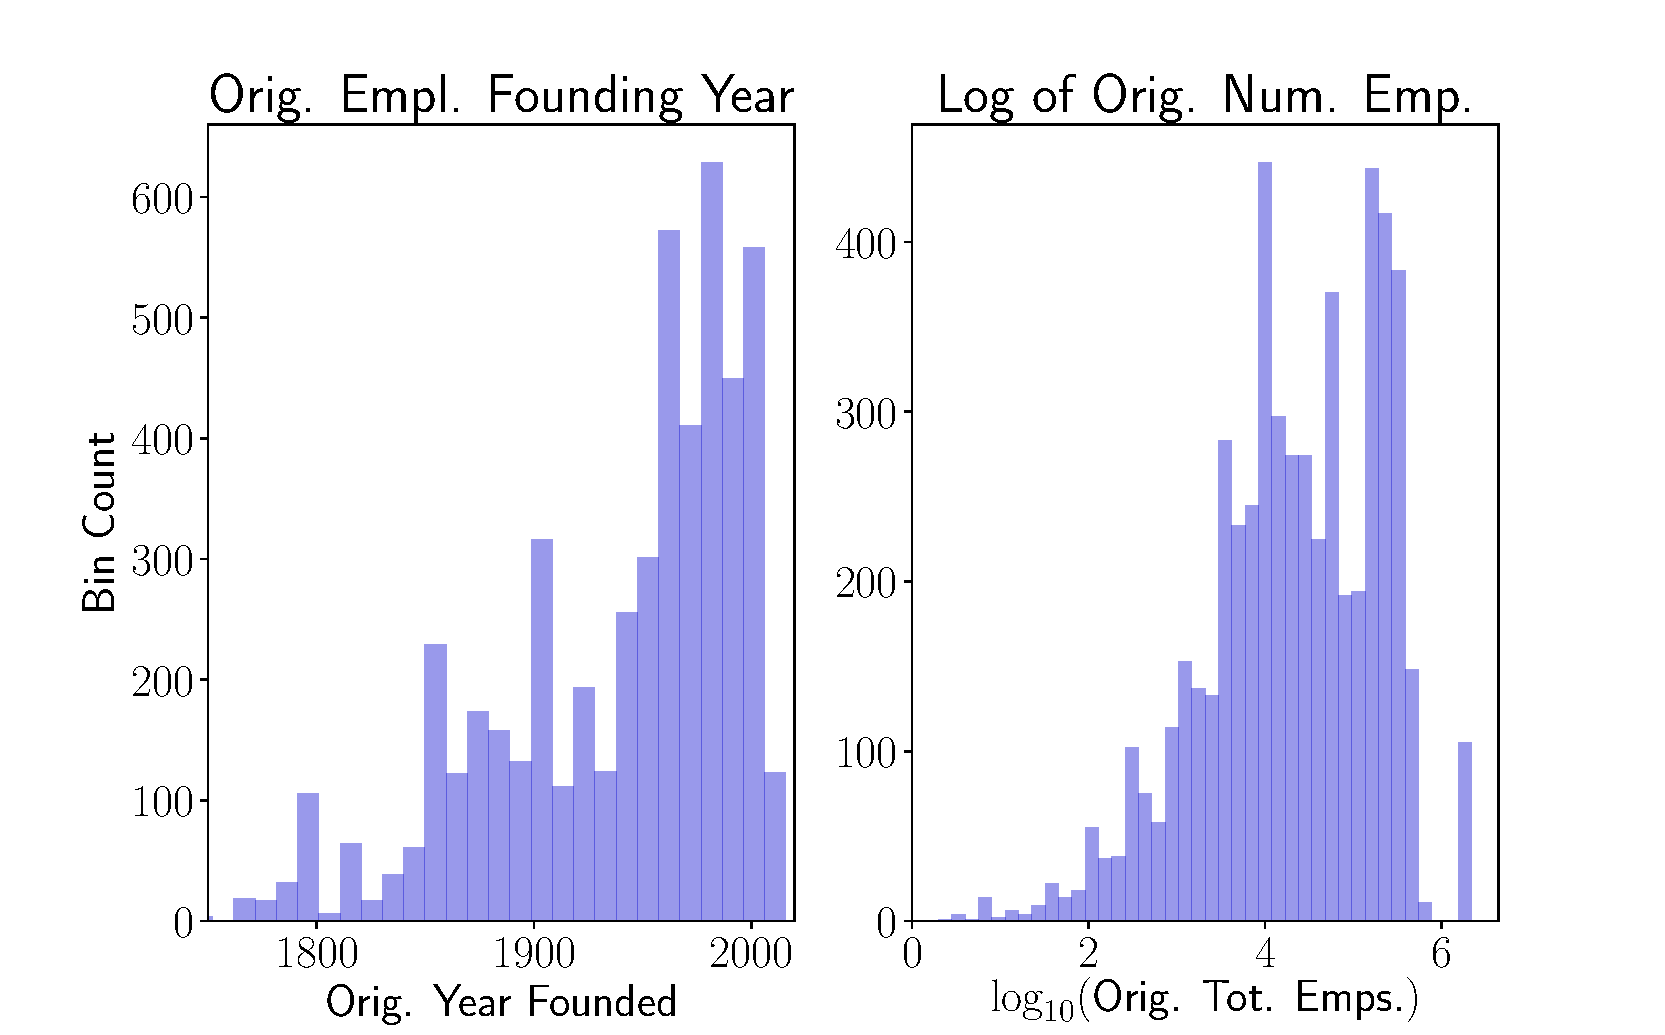
\includegraphics[width=1.0\linewidth]{emplstat.pdf}
    %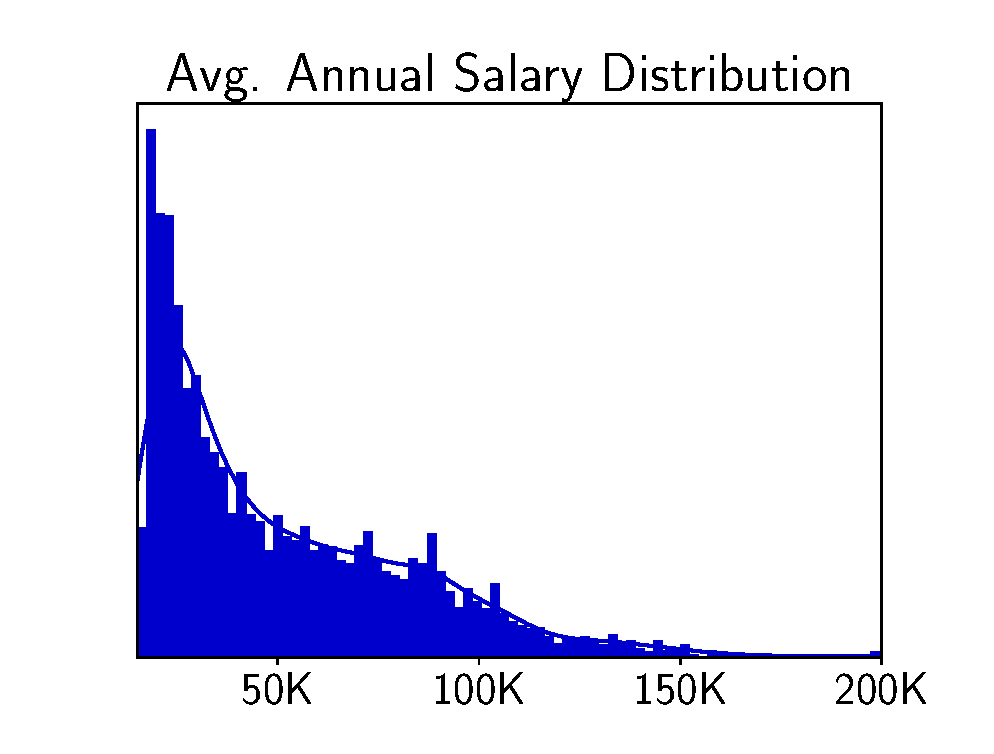
\includegraphics[trim={3cm 3cm 3cm 3cm}, clip,width=0.9\linewidth]{avgsal.eps}
	\caption{Original employer founding year and employee number distributions}
	\label{fig:emplstat}
\end{figure}


\begin{figure}[thb]
    \centering
	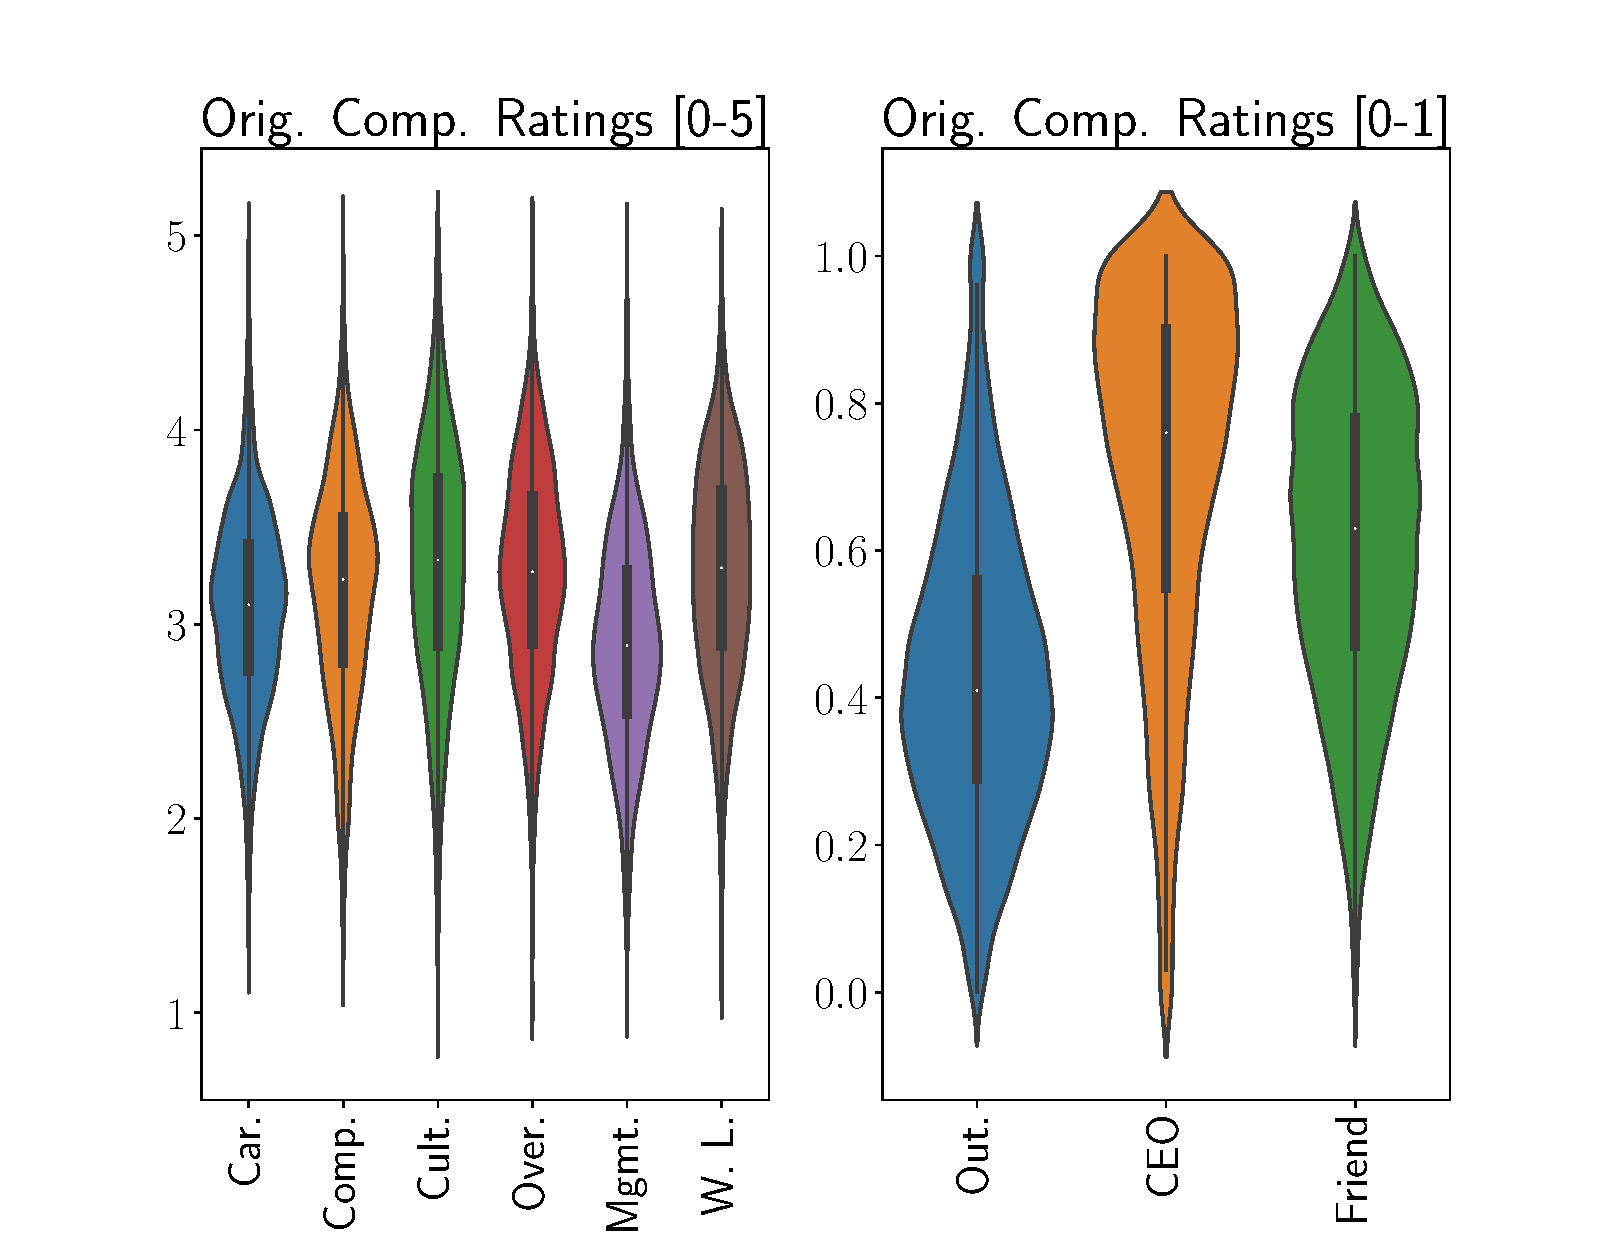
\includegraphics[width=1.0\linewidth]{vioplt.pdf}
    %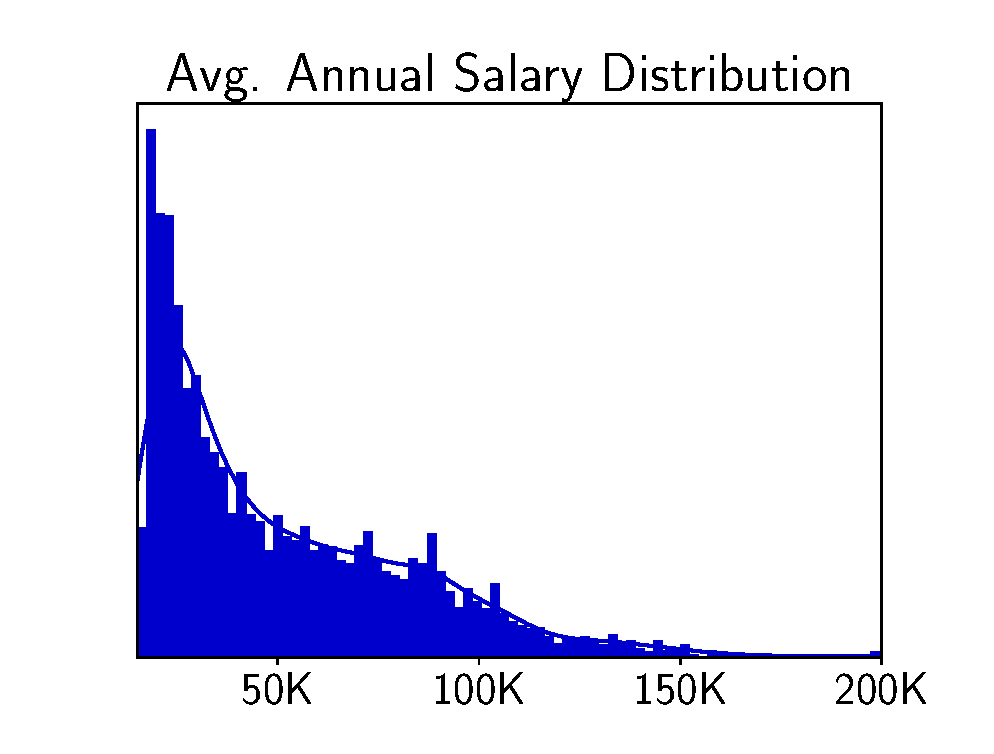
\includegraphics[trim={3cm 3cm 3cm 3cm}, clip,width=0.9\linewidth]{avgsal.eps}
	\caption{Violin Plots ... }
	\label{fig:vioplt}
\end{figure}


Quantile normalization ... others 

Feature engineering 
\begin{enumerate}
    \item percentage increase in salary 
\end{enumerate}

\section{Exploratory Insights}

Sum. 

\subsection{Idea 1}


\subsection{Idea 2}

\section{Towards an Attrition Model}

adf

\subsection{Linear Review}


\subsection{Logistic Work}


\subsection{Binary Classifier}

\subsection{Model Performance Comparison}

\section{Conclusions and Extensions}


Here we describe several ideas to pursue as part of this study

Mention limitations here (same as in glassdoor article and others that we find) ... then 
mention that our extensions will overcome these limitations 

-- company specific analytics
-- competative analysis
-- linkedin, full glassdoor dataset 
-- outlier determination may serve as a glassdoor fake review filter 


% For one-column wide figures use
%\begin{figure}[thb]
	% Use the relevant command to insert your figure file.
	% For example, with the graphicx package use
%    \centering
%	
\includegraphics[trim={3cm 3cm 3cm 3cm}, clip,width=0.9\linewidth]{sample-image}
	% figure caption is below the figure
%	\caption{Sample figure with caption.}
%	\label{fig: sample-figure}       % Give a unique label
%\end{figure}

\textbf{Acknowledgements:} The authors would like to ack... for sharing data FINISH WHEN DONE

% if added before the last page, this command can help balancing columns
%\addtolength{\textheight}{-.2cm} 

%Bibliography 
\bibliographystyle{ieeetr}
\bibliography{sample}

\begin{enumerate}
    \item Old to new industry ... matrix here 
    \item Let's focus on Leaving a company, not just different role in same company 
    \item Look at rankings from old company to new one; what can we say overall about 
         the characteristics of these companies?  What factors did we see the most signi
         change in? Make scatter plots/hists here 
    \item job title transition? progression ... Markov chain? 
    \item What other summary statistics are relevant that go beyond what is already in 
          the Glassdoor article? 
    \item Do a brief literature review.  What has been done in this area already?
          Summarize Glassdoor as part of this ... describe the uniqueness of this dataset. 
          Mention it would be of interest to expand ... mine LinkedIn as well to do a 
          more thorough study later. 
    \item do reasons vary by length of job??? 
    \item Look at people who made a major change (e.g. shifted geographic regions. ... more than 500 miles 
          away ... is motivation any different for these people?)
    \item Look at how old vs new ranking variable scatter plots differ from the y=x line, 
        e.g. if employees change, which variables to we find also change significantly?  
          Do some change always in the upwards direction? Linear reg. essentially tries 
          to understand to what extent is this line differs from 1, e.g. if it is 1 for 
          a given variable, then this variable has no influence ... can we develop a 
          better variable influence measure here? 
    \item Look at people who switched industries ... any different motivation here? 
    \item One interesting feature is that employees seldom seem to stay at a company that has the 
          same size as their old one.  Lots of shirts from large to small or vice versa.  Perhaps 
          make this more quantitative? 
    \item  check if job-len corresponds to start,end date difference 
    \item Any info associated with geographic studies?  Large vs small cities? 
    \item  patterns that stem from either age or employment tenure? 
    \item binary model classifer, ROC curve etc. 
    \item impl their original regression model ... test 
    \item  industry specific studies 
    \item Distribution of dates that changes were made ... do we see a pattern on times of the 
          year that moves occurred 
    \item explore patterns between old and new firms using year founded 
\end{enumerate}

\end{document}


\end{document}
